% 2009 年陕西卷文科第 19 题：直三棱柱 ABC-A1B1C1（AB=1，AC=AA1=√3，∠ABC=60°）。
% 来源 PDF：普通高考/2009/2009陕西文.pdf，SHA-256 c4760285004d01aee97af7821783660b08339cca3a3fc8645052f11001ba586a。
% 原页：第 1 页（A3 三栏）第 3 栏下部，书页码 551。
% 重绘依据：B(0,0,0)、A(1,0,0)、C(1,√3,0)、A1(1,0,√3)，投影 (x,y,z)->(x+0.35y, 1.6z+0.25y)。
%   A1C 为解题辅助线，画虚线；其余棱按直三棱柱绘制。
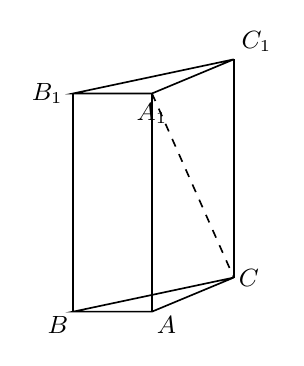
\begin{tikzpicture}[semithick, every node/.style={inner sep=1.5pt, font=\small}]
  \coordinate (B)  at (0.000,0.000);
  \coordinate (A)  at (1.000,0.000);
  \coordinate (C)  at (2.039,0.433);
  \coordinate (B1) at (0.000,2.771);
  \coordinate (A1) at (1.000,2.771);
  \coordinate (C1) at (2.039,3.204);

  % 棱
  \draw (B) -- (A) -- (C) -- cycle;
  \draw (B1) -- (A1) -- (C1) -- cycle;
  \draw (A) -- (A1);
  \draw (B) -- (B1);
  \draw (C) -- (C1);
  % 辅助线
  \draw[dashed] (A1) -- (C);

  % 标注
  \node[below left] at (B) {$B$};
  \node[below right] at (A) {$A$};
  \node[right] at (C) {$C$};
  \node[left=2pt] at (B1) {$B_1$};
  \node[below=2pt] at (A1) {$A_1$};
  \node[above right=1pt] at (C1) {$C_1$};
\end{tikzpicture}
